\documentclass[compress]{beamer}
\usepackage{ifthen,verbatim}

\title{Muon Alignment Quality \\ on the Eve of the CSA08 Exercise}
\author{Jim Pivarski, Alexei Safonov, K\'aroly Banicz$^*$}
\institute{Texas A\&M University, $^*$FermiLab}
\date{ 8 May, 2008}

\newcommand{\isnote}{}
\xdefinecolor{lightyellow}{rgb}{1.,1.,0.25}
\xdefinecolor{darkblue}{rgb}{0.1,0.1,0.7}

%% Uncomment this to get annotations
%% \def\notes{\addtocounter{page}{-1}
%%            \renewcommand{\isnote}{*}
%% 	   \beamertemplateshadingbackground{lightyellow}{white}
%%            \begin{frame}
%%            \frametitle{Notes for the previous page (page \insertpagenumber)}
%%            \itemize}
%% \def\endnotes{\enditemize
%% 	      \end{frame}
%%               \beamertemplateshadingbackground{white}{white}
%%               \renewcommand{\isnote}{}}

%% Uncomment this to not get annotations
\def\notes{\comment}
\def\endnotes{\endcomment}

\setbeamertemplate{navigation symbols}{}
\setbeamertemplate{headline}{\mbox{ } \hfill
\begin{minipage}{5.5 cm}
\vspace{-0.75 cm} \small
\end{minipage} \hfill
\begin{minipage}{4.5 cm}
\vspace{-0.75 cm} \small
\begin{flushright}
\ifthenelse{\equal{\insertpagenumber}{1}}{}{Jim Pivarski \hspace{0.2 cm} \insertpagenumber\isnote/\pageref{numpages}}
\end{flushright}
\end{minipage}\mbox{\hspace{0.2 cm}}\includegraphics[height=1 cm]{../cmslogo} \hspace{0.1 cm} \includegraphics[height=1 cm]{../tamulogo} \hspace{0.01 cm} \vspace{-1.05 cm}}

\begin{document}
\frame{\titlepage}

%% \begin{notes}
%% \item This is the annotated version of my talk.
%% \item If you want the version that I am presenting, download the one
%% labeled ``slides'' on Indico (or just ignore these yellow pages).
%% \item The annotated version is provided for extra detail and a written
%% record of comments that I intend to make orally.
%% \item Yellow notes refer to the content on the {\it previous} page.
%% \item All other slides are identical for the two versions.
%% \end{notes}

\begin{frame}
\frametitle{Outline}
\begin{itemize}\setlength{\itemsep}{0.75 cm}
\item Nutshell history since CSA07
\item Which ``baseline'' procedure is best (which should we use in CSA08)?
\item Dependence of alignment quality on initial misalignment
\item Status of the overlap procedure for beam-halo and cosmic rays
\item Workflows in CSA08
\end{itemize}
%% \hspace{-0.83 cm} \textcolor{darkblue}{\Large Outline2}
\end{frame}

\begin{frame}
\frametitle{Quick history (1/2)}

\small
\begin{itemize}
\item Last year, we developed an ``infinite APE'' technique for
aligning the muon system:
\begin{enumerate}
\item refit globalMuons with unphysically large Alignment Position Errors on the muon hits
\item resulting track is dominated by tracker information, but we can calculate muon residuals
\item converges in one iteration because we're using external information
\end{enumerate}
\item CSA07 exercise included an event sample which was misaligned at the RECO level

\mbox{ } \hfill 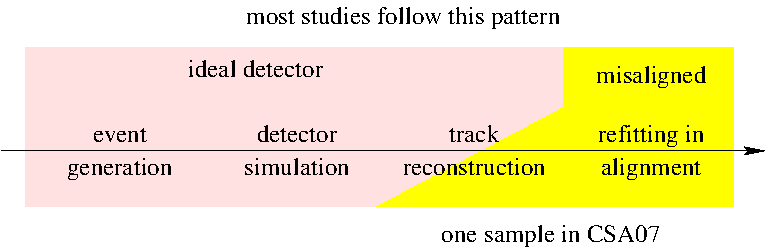
\includegraphics[width=0.6\linewidth]{misal_at_reco.pdf} \hfill \mbox{ }

\begin{itemize}
\item revealed that apparent prior success was due to an incomplete
re-fit, and the track deviously carried information about the ideal detector (except in CSA07)
\end{itemize}
\end{itemize}
\end{frame}

\begin{frame}
\frametitle{Quick history (2/2)}

\small
\begin{itemize}
\item Correcting that mistake led to poor alignment results because we
were dealing with the full alignment problem for the first time,
including extrapolation errors due to multiple scattering
\item We quickly modified our procedure to take advantage of local information:
\begin{enumerate}
\item align only station 1 in the first stage
\item fit tracks with tighter APEs in station 1 and align station 2\ldots
\end{enumerate}

\item In early tests, ``staged procedure'' did better than ``infinite
APE'', so I developed this procedure in earnest, yielding 0.4--1.6~mm
resolution on chamber resolution in most stations

\item In my early tests, I conflated ``infinite APE'' with ``track
propagated from tracker'' which naively should be the same thing, but
there are differences which lead to alignment error

\item Many bug-fixes later (both procedures improved), I find that the
real ``infinite APE'' yields the best results: 0.2--0.7~mm

\item But it also depends on degree of initial misalignment

\end{itemize}
\end{frame}

\begin{frame}
\frametitle{New results}

\begin{itemize}\setlength{\itemsep}{0.25 cm}
\item First, I want to show are the new results with the real ``infinite APE'' technique.

\item These come from a pre-CSA test (1\_8\_4 FastSim) with
7~pb$^{-1}$ of $W\to\mu\nu$

\item Chambers start with the 0~pb$^{-1}$ misalignment scenario and
no misaligned layers

\item (These are in publicity-plot form, which will be filled with
CSA08 results in two weeks)
\end{itemize}

\end{frame}

\begin{frame}
\frametitle{New Barrel \only<1>{aligned positions}\only<2>{track residuals}}

\only<1>{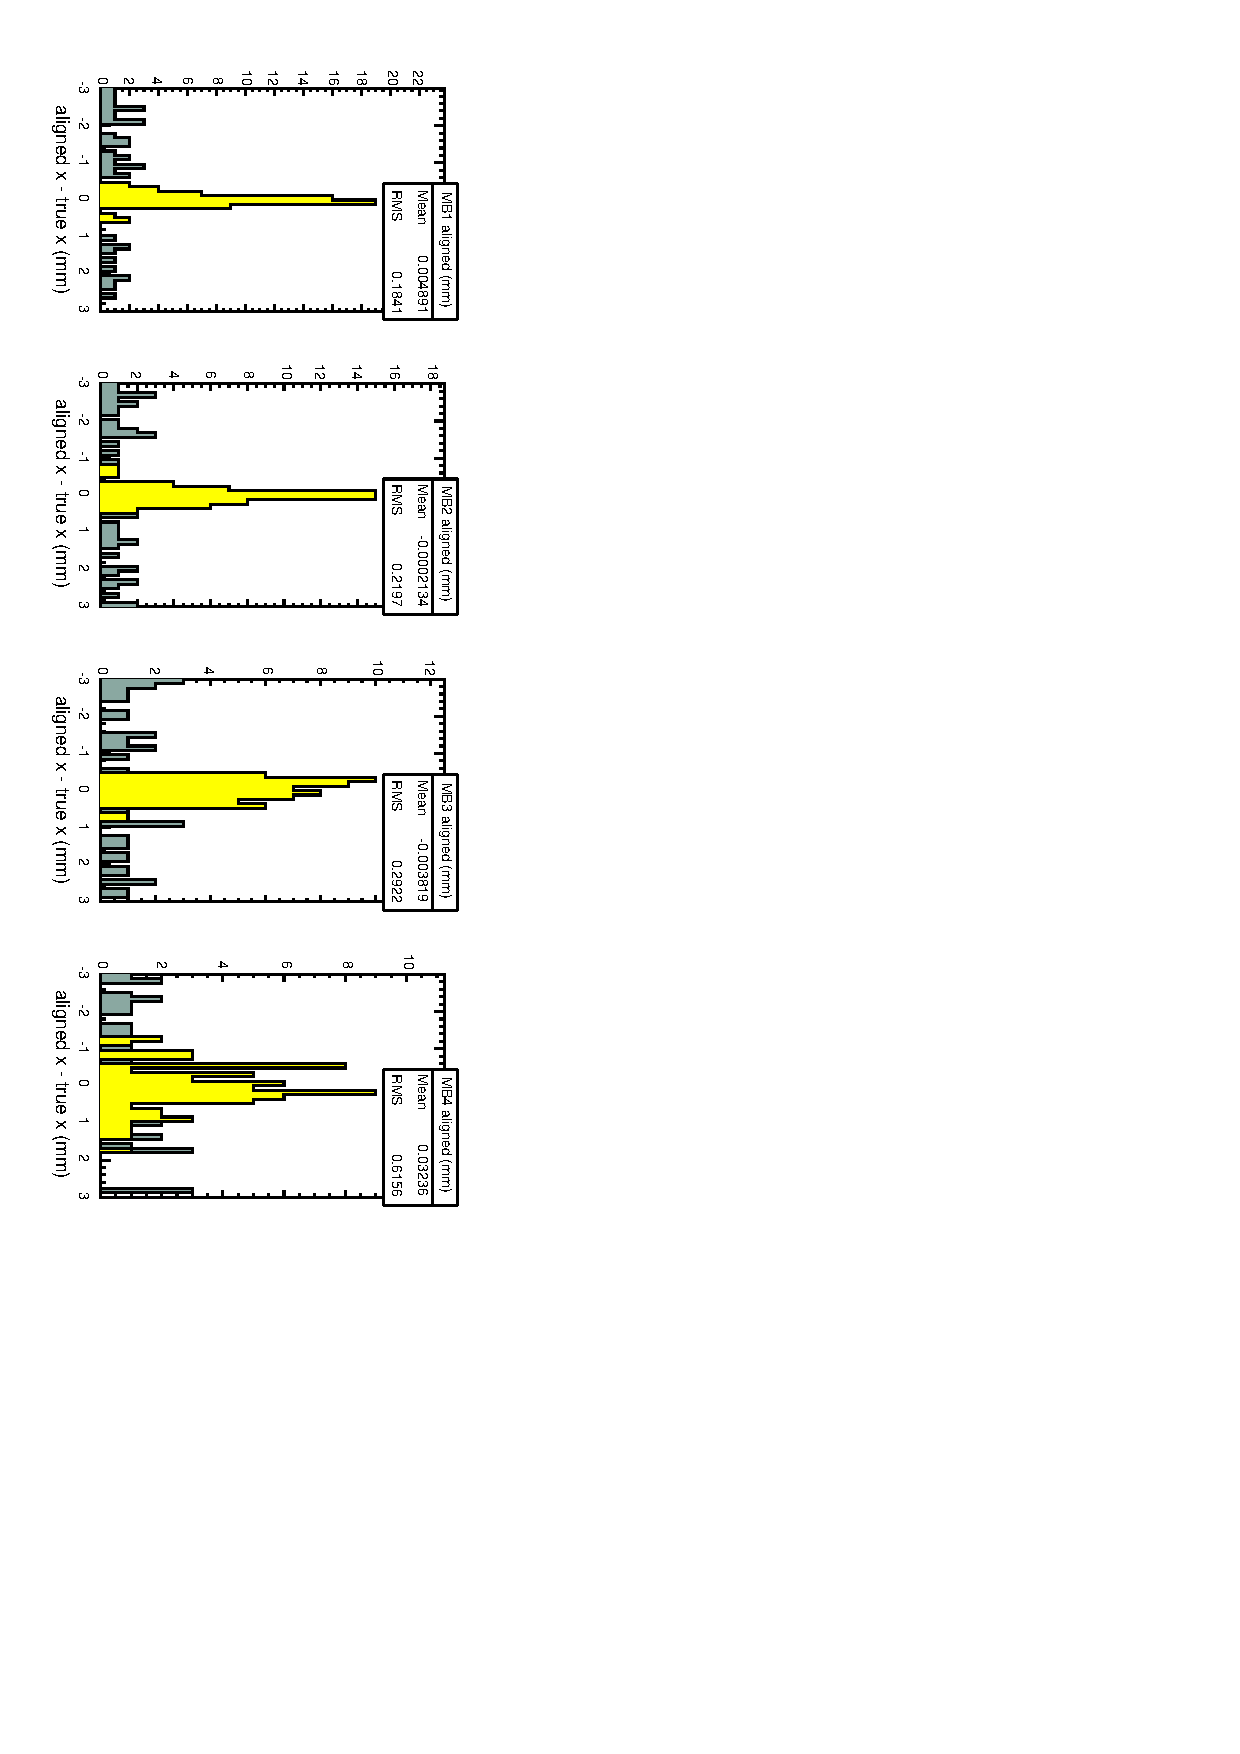
\includegraphics[height=\linewidth, angle=90]{barrel_184.pdf}}
\only<2>{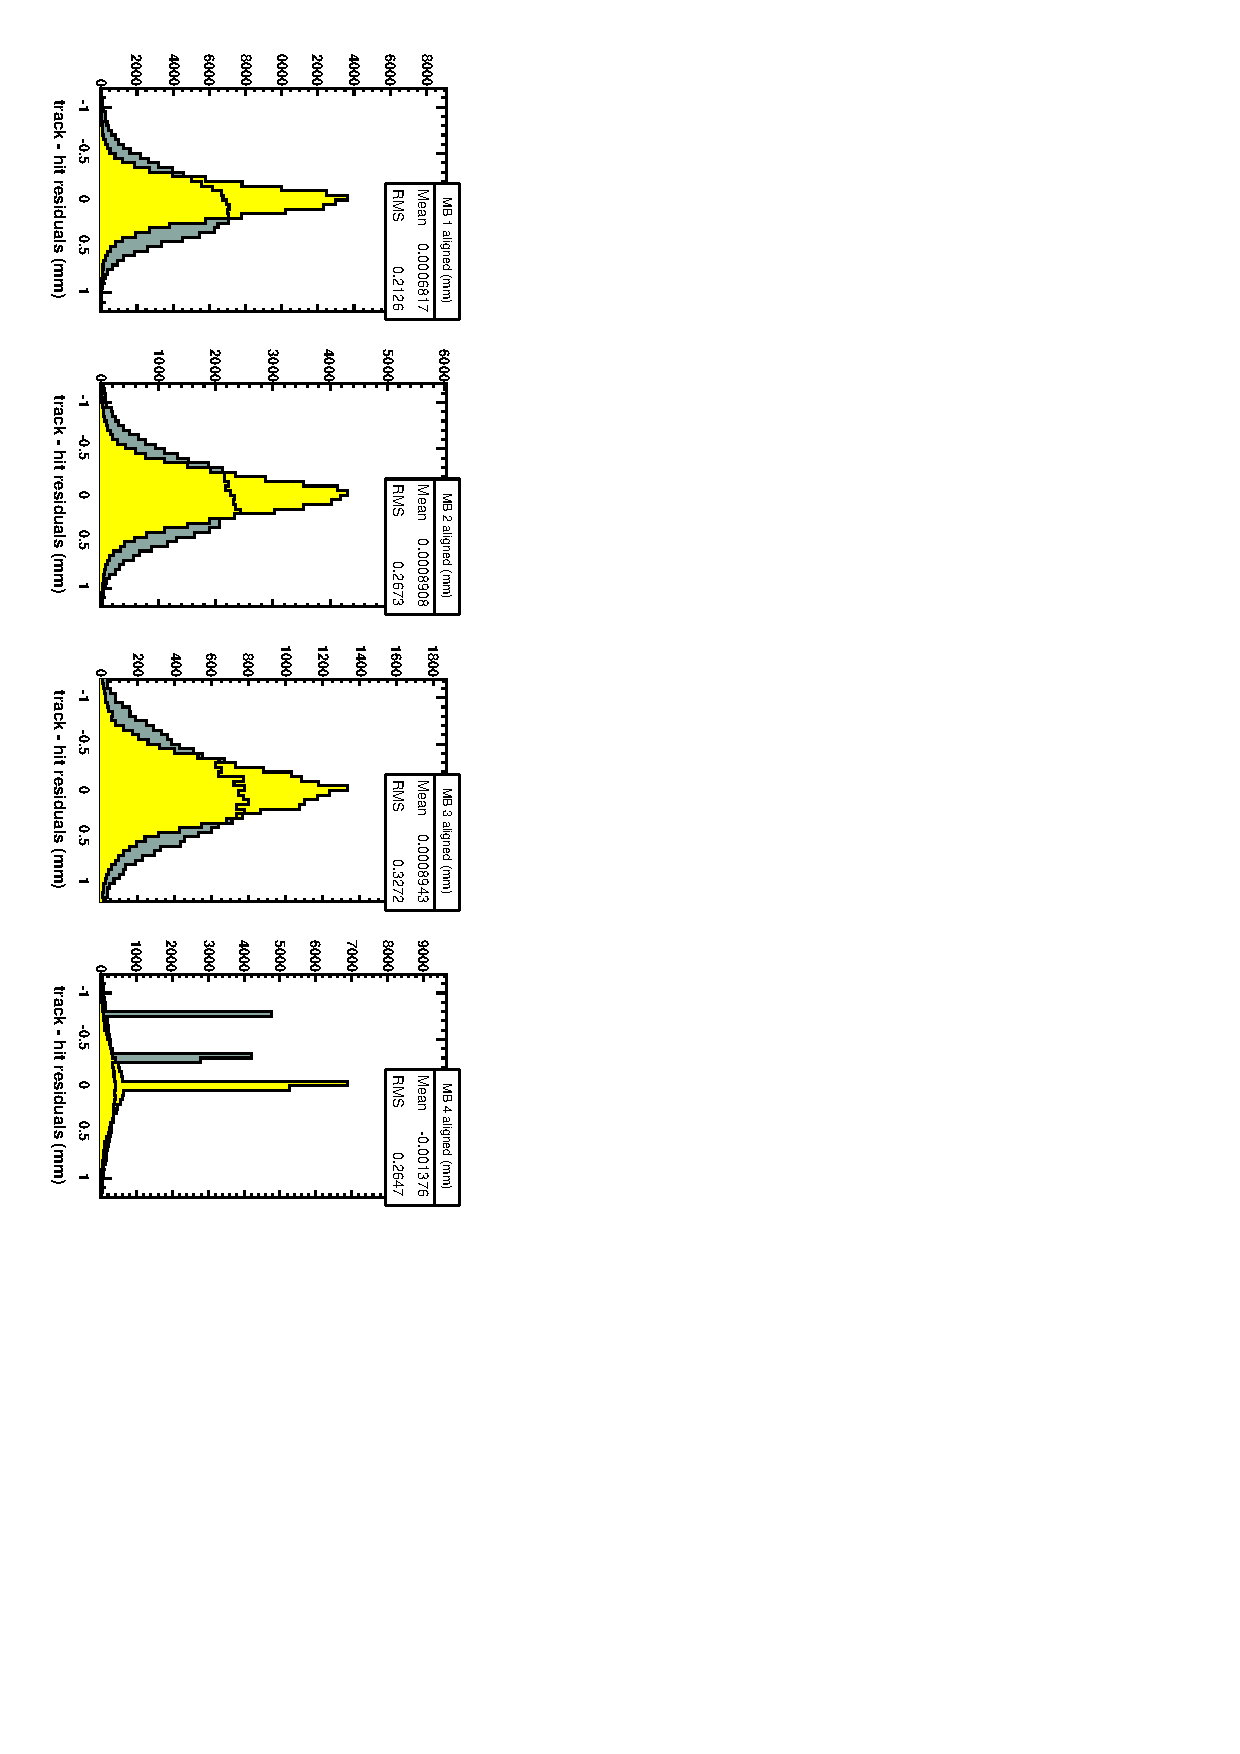
\includegraphics[height=\linewidth, angle=90]{barrel_resid_184.pdf}}

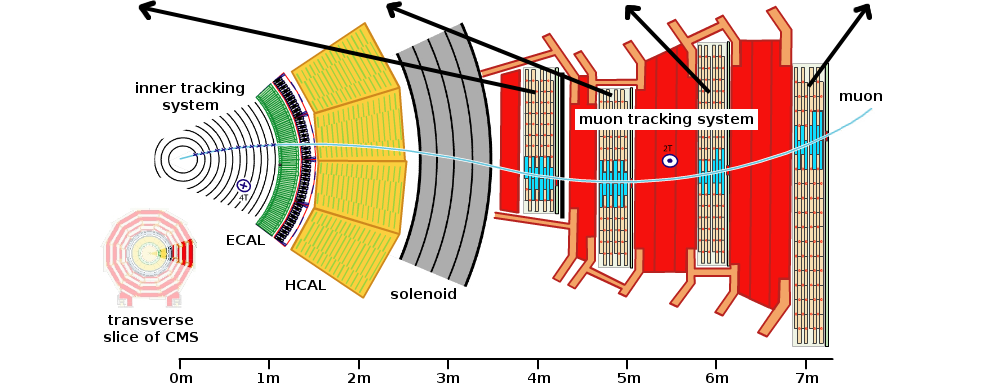
\includegraphics[width=\linewidth]{cms_slice.png}
\end{frame}

\begin{frame}
\frametitle{New Endcap \only<1>{aligned positions}\only<2>{track residuals}}

\begin{columns}
\column{0.35\linewidth}
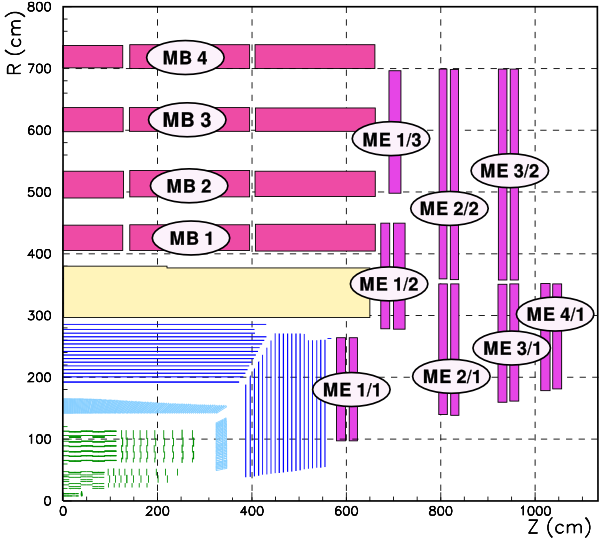
\includegraphics[width=\linewidth]{muon_system.png}
\column{0.8\linewidth}
\only<1>{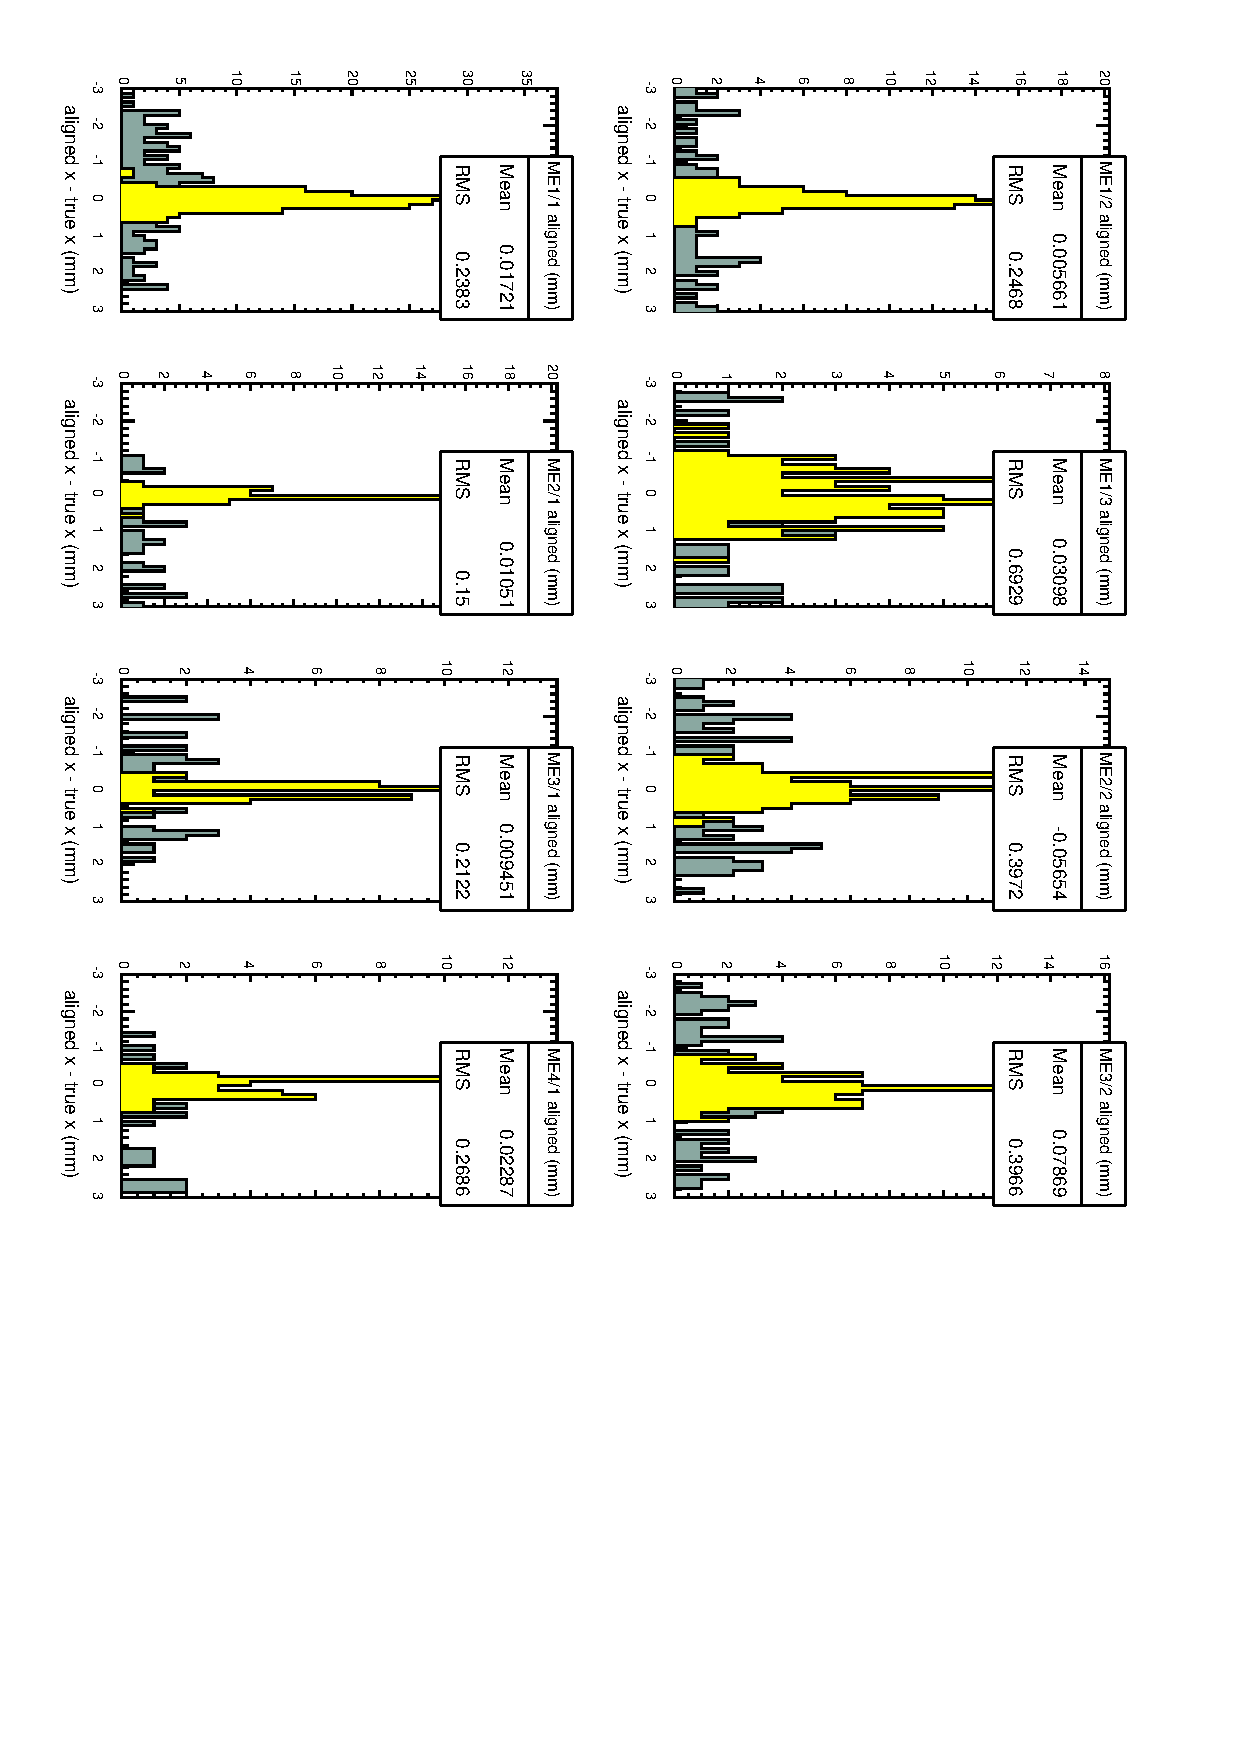
\includegraphics[height=\linewidth, angle=90]{endcap_184.pdf}}
\only<2>{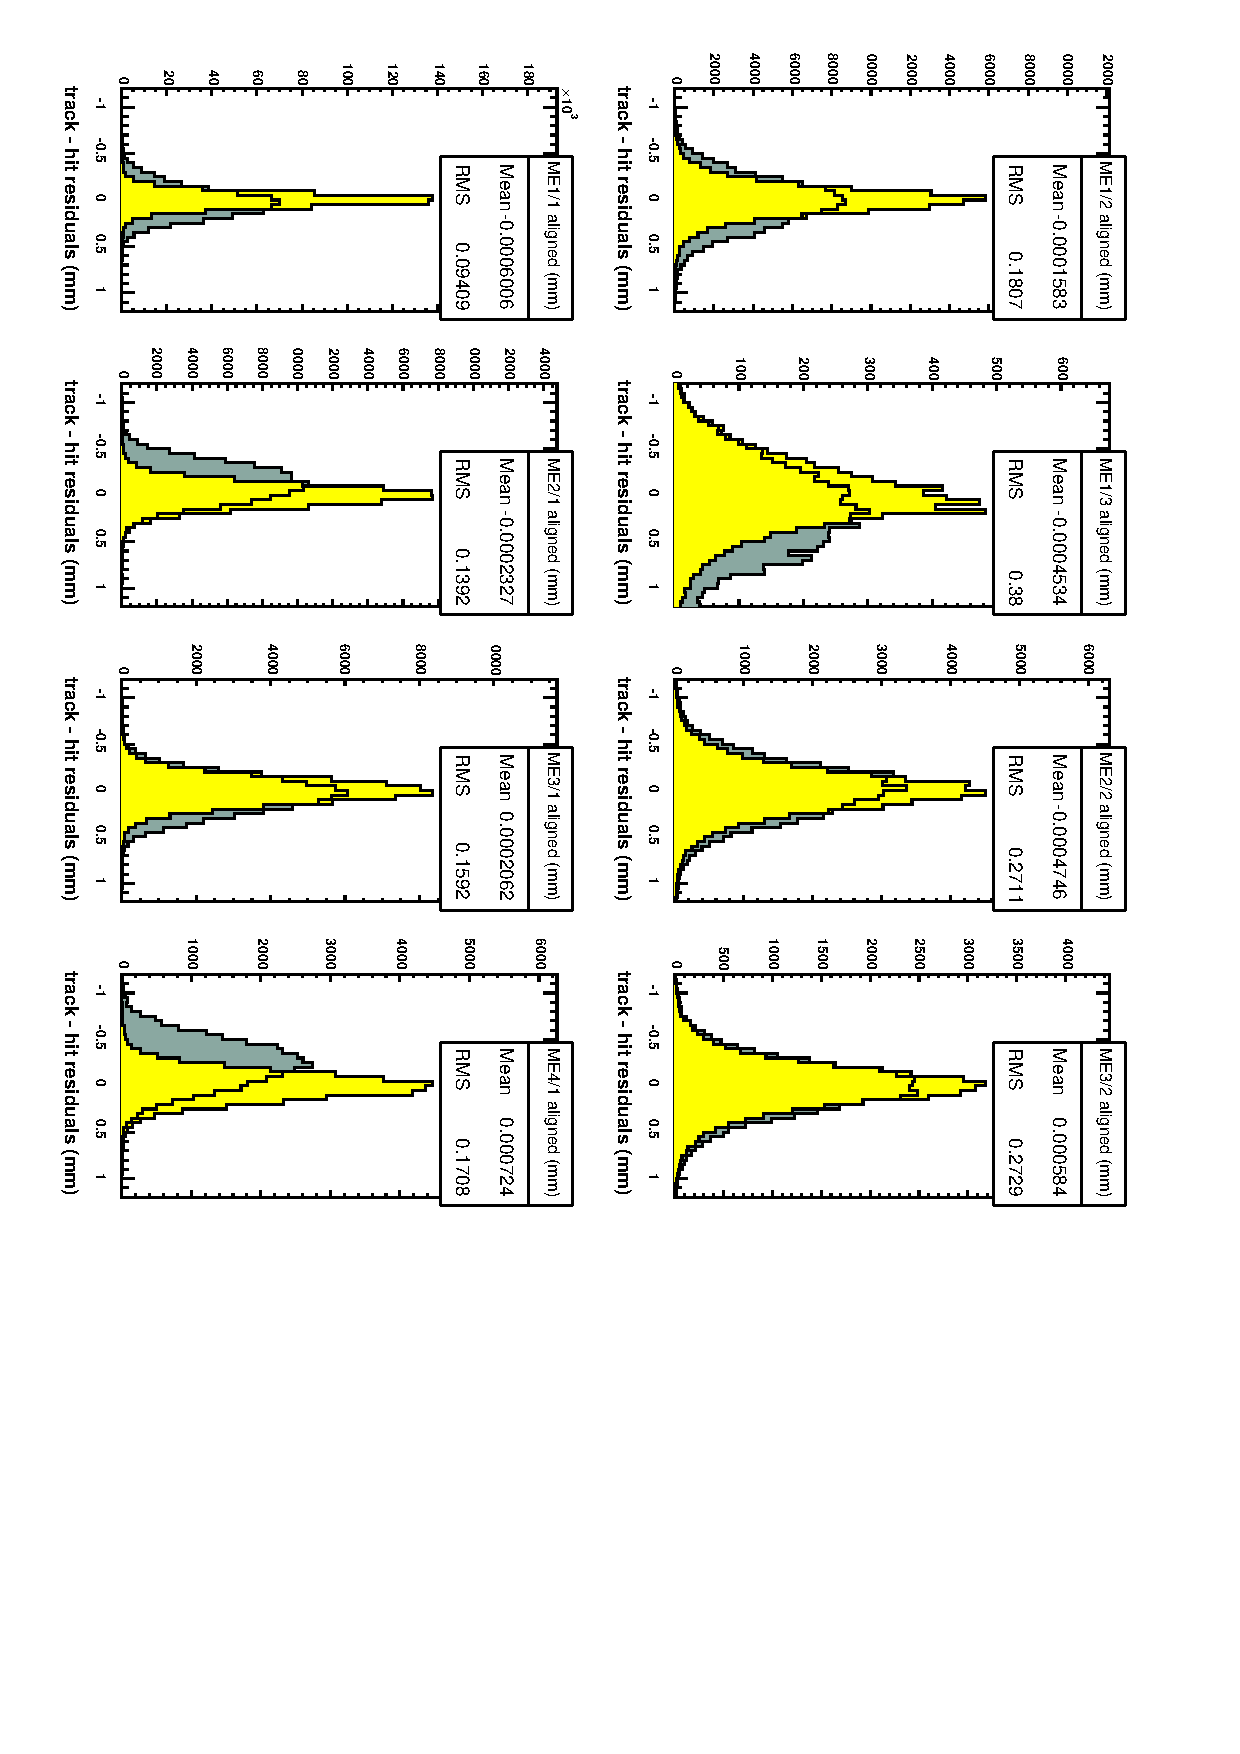
\includegraphics[height=\linewidth, angle=90]{endcap_resid_184.pdf}}
\end{columns}

\end{frame}

\begin{frame}
\frametitle{``Infinite APE'' is good again?}

\small

\begin{itemize}
\item High-quality results from ``infinite APE'' made me suspicious,
because this is the procedure that suffered from the ``devious tracks'' bug
\item Are the tracks remembering the RECO geometry now?  Test:
\begin{enumerate}
\item Rotate tracker by 1~mrad, refit tracks
\item Check $\phi$ of each track extrapolation, track-by-track,
surface-by-surface: the difference should always be 1~mrad
\end{enumerate}
\end{itemize}

\mbox{ } \hfill 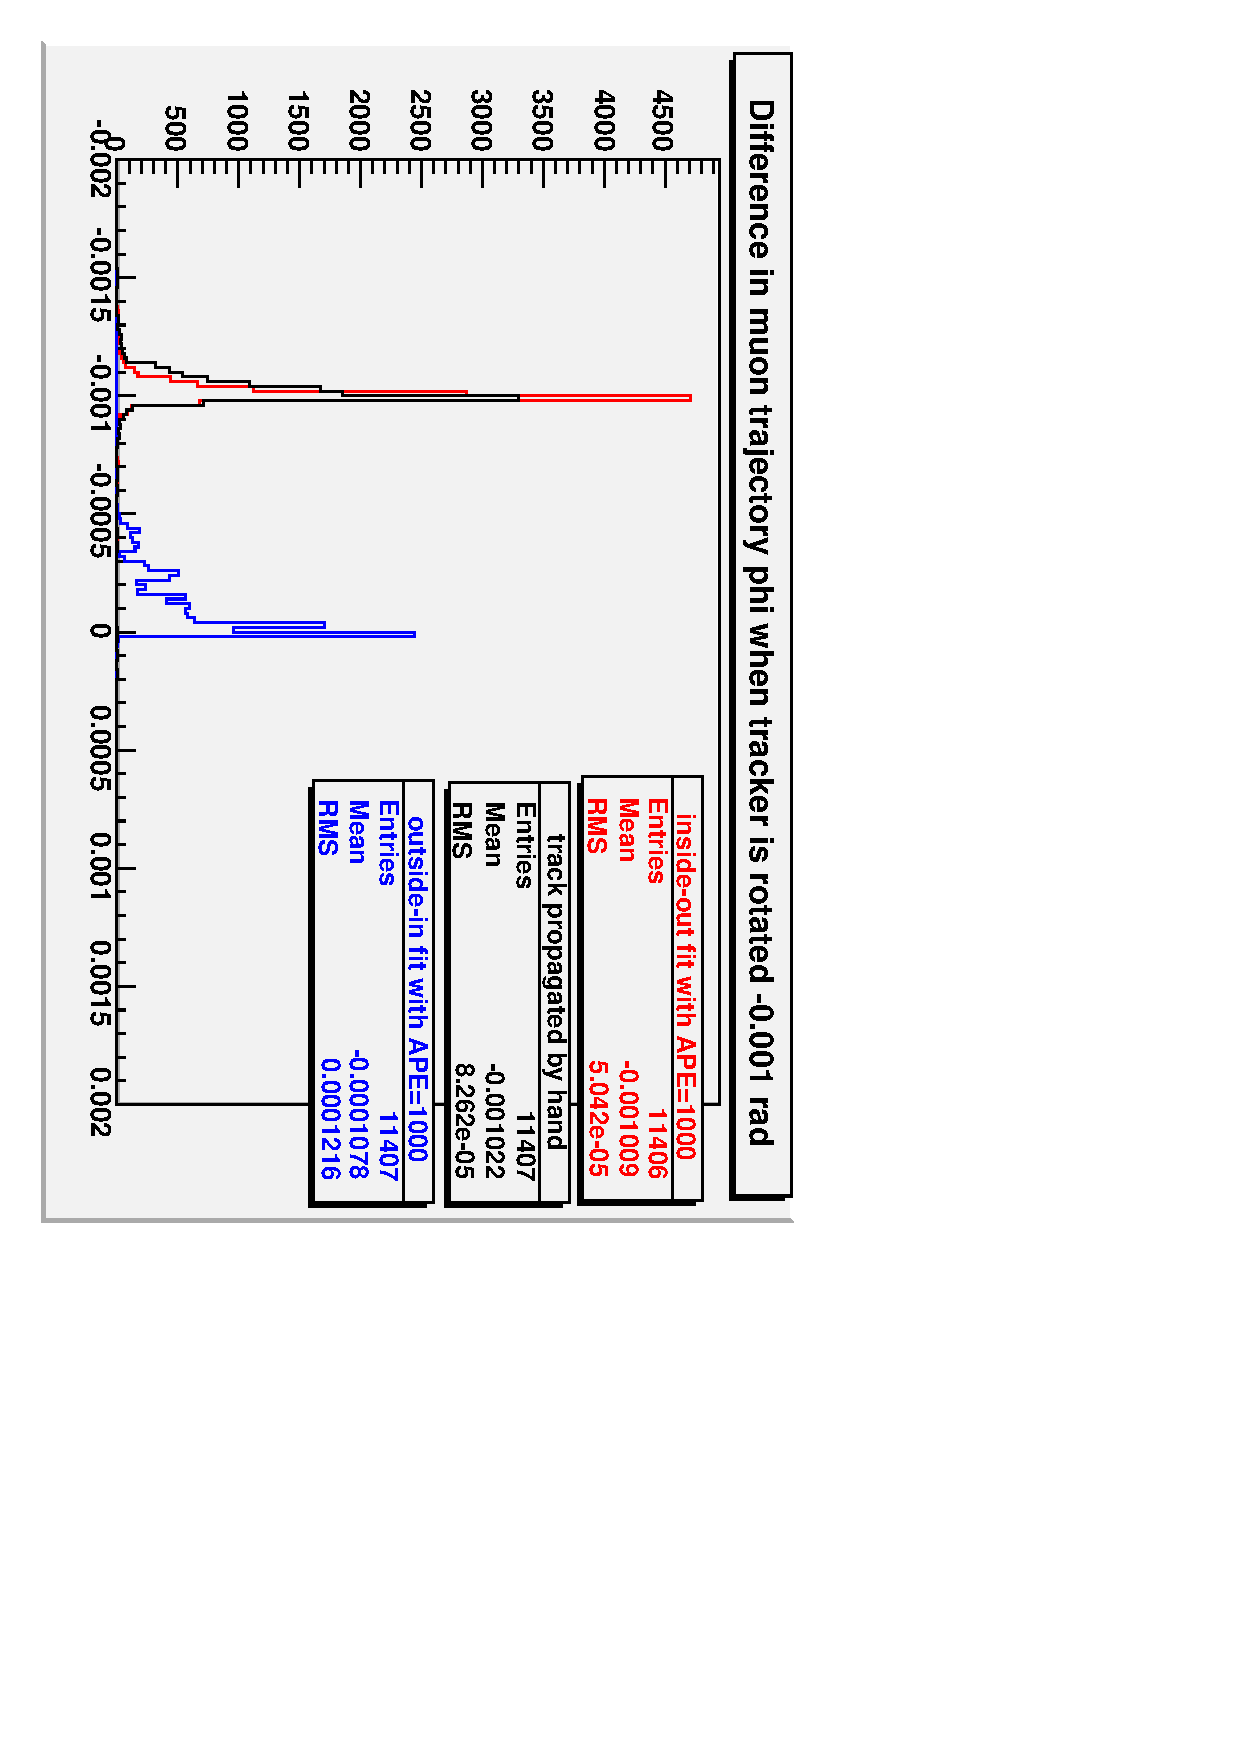
\includegraphics[height=0.7\linewidth, angle=90]{phi_propagation_differences.pdf} \hfill \mbox{ }
\end{frame}

\begin{frame}
\frametitle{``Infinite APE'' is good again?}

\small

\begin{itemize}
\item Tracks remembered RECO geometry when refit \textcolor{blue}{from the outside-in}
\item We now always fit \textcolor{red}{from the inside-out}
\item Black curve: calling the propagator directly to extrapolate from tracker to muon system
\begin{itemize}
\item Naively, this should be the same as infinite APE
\item There are small differences, even after correcting a
firstMeasurement()/lastMeasurement() mistake in my code
\item I based my decision to pursue the ``staged approach'' on results
from the propagator, which is different enough to yield a factor of 2
worse alignment resolution ($\Delta \phi$ of 0.001 $\to$ $\sim$5~mm)
\end{itemize}
\end{itemize}

\mbox{ } \hfill 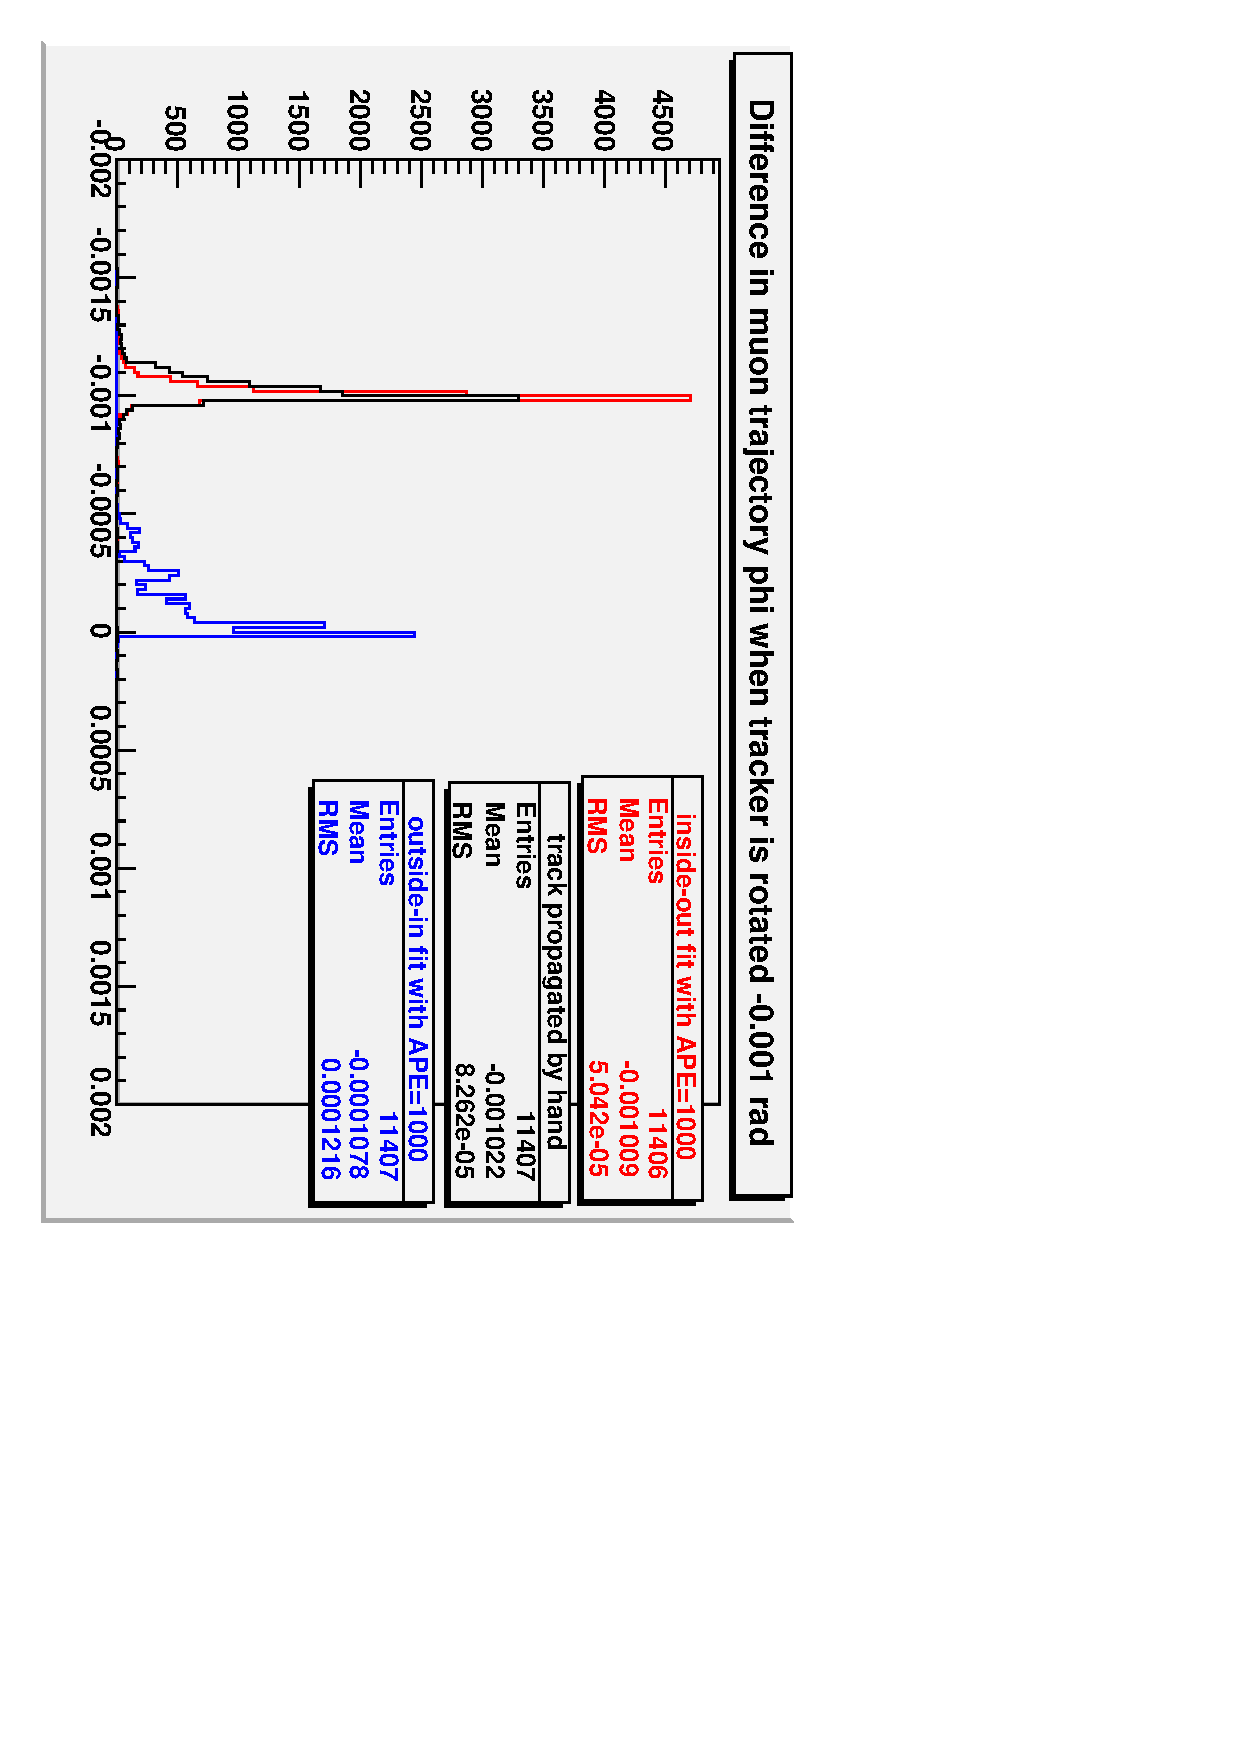
\includegraphics[height=0.5\linewidth, angle=90]{phi_propagation_differences.pdf} \hfill \mbox{ }
\end{frame}

\begin{frame}
\frametitle{Staged procedure}

\small

Current state of the staged procedure versus iteration (100~pb$^{-1}$):

\vfill
\begin{columns}
\column{0.5\linewidth}
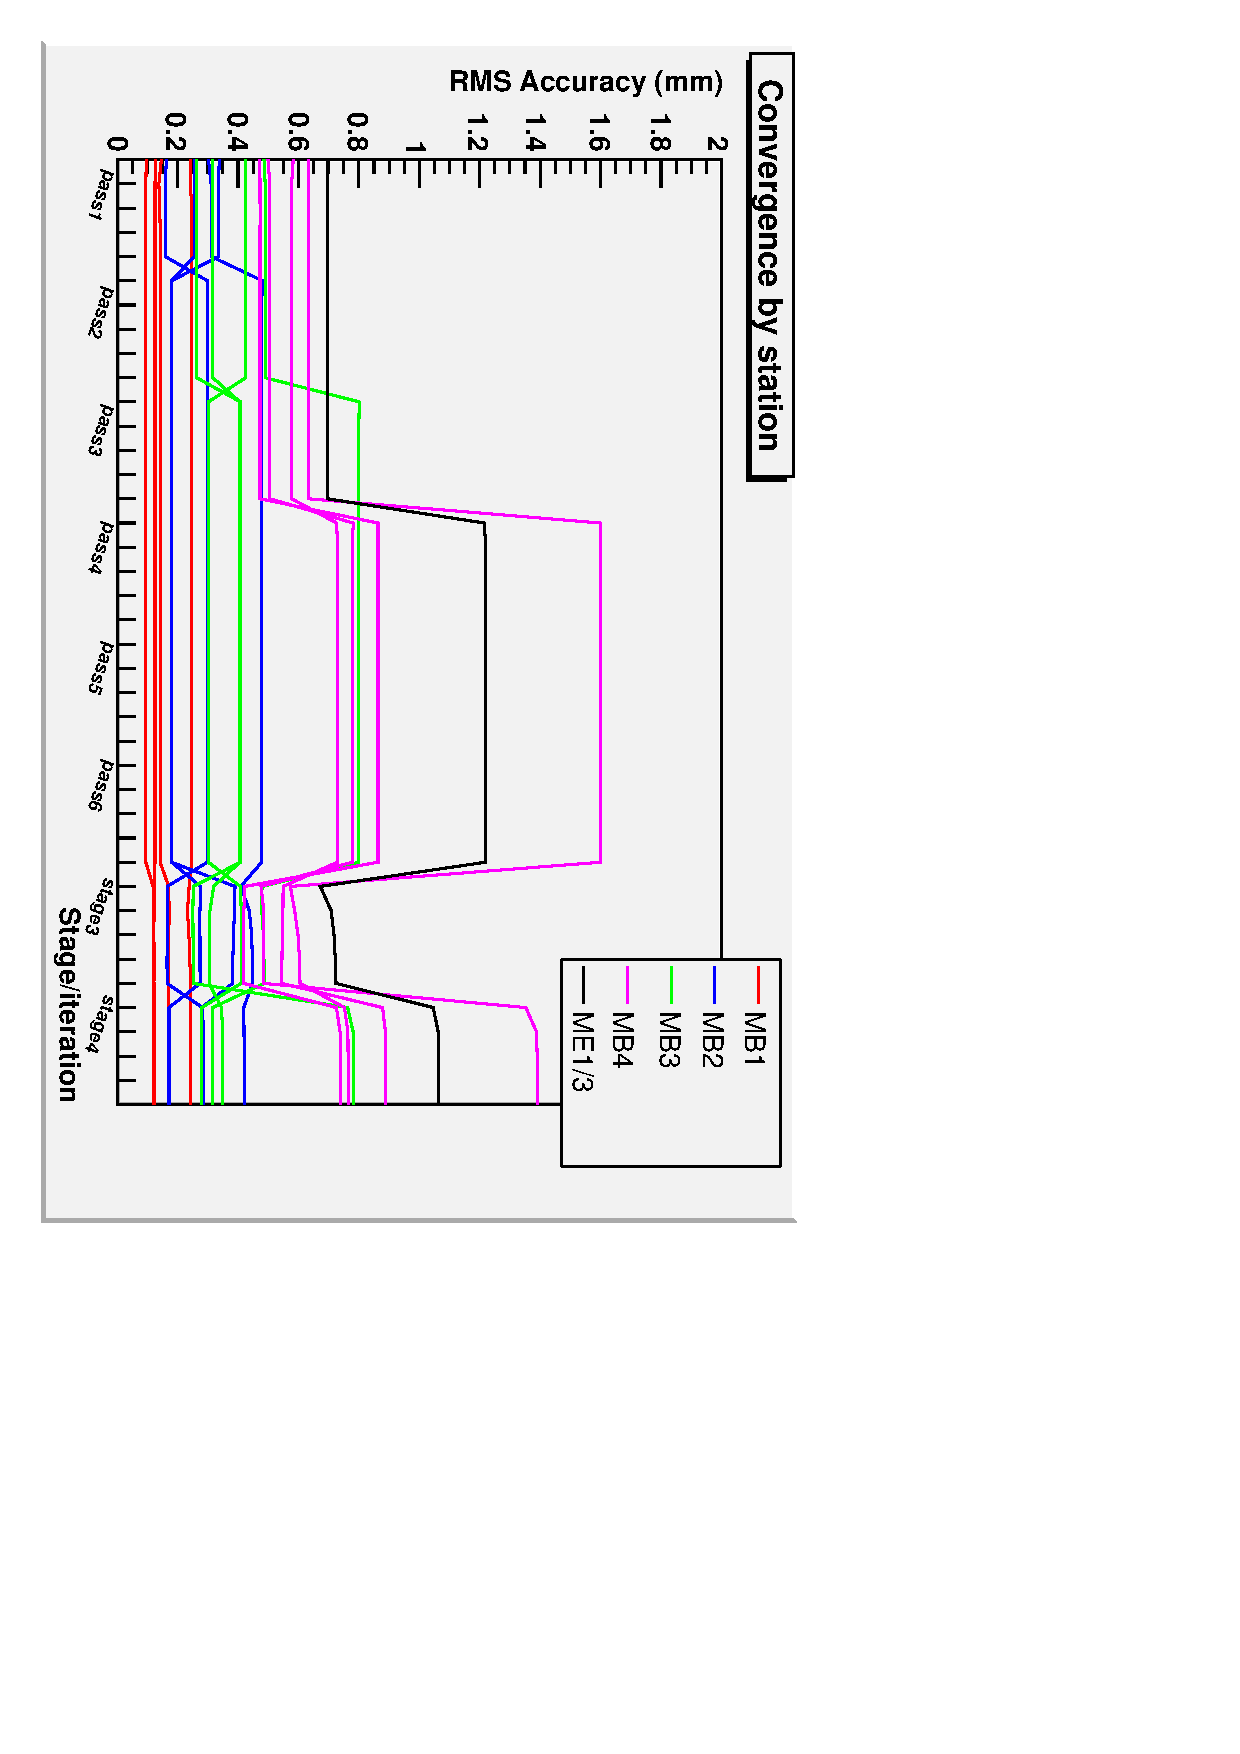
\includegraphics[height=\linewidth, angle=90]{convergence_barrel.pdf}
\column{0.5\linewidth}
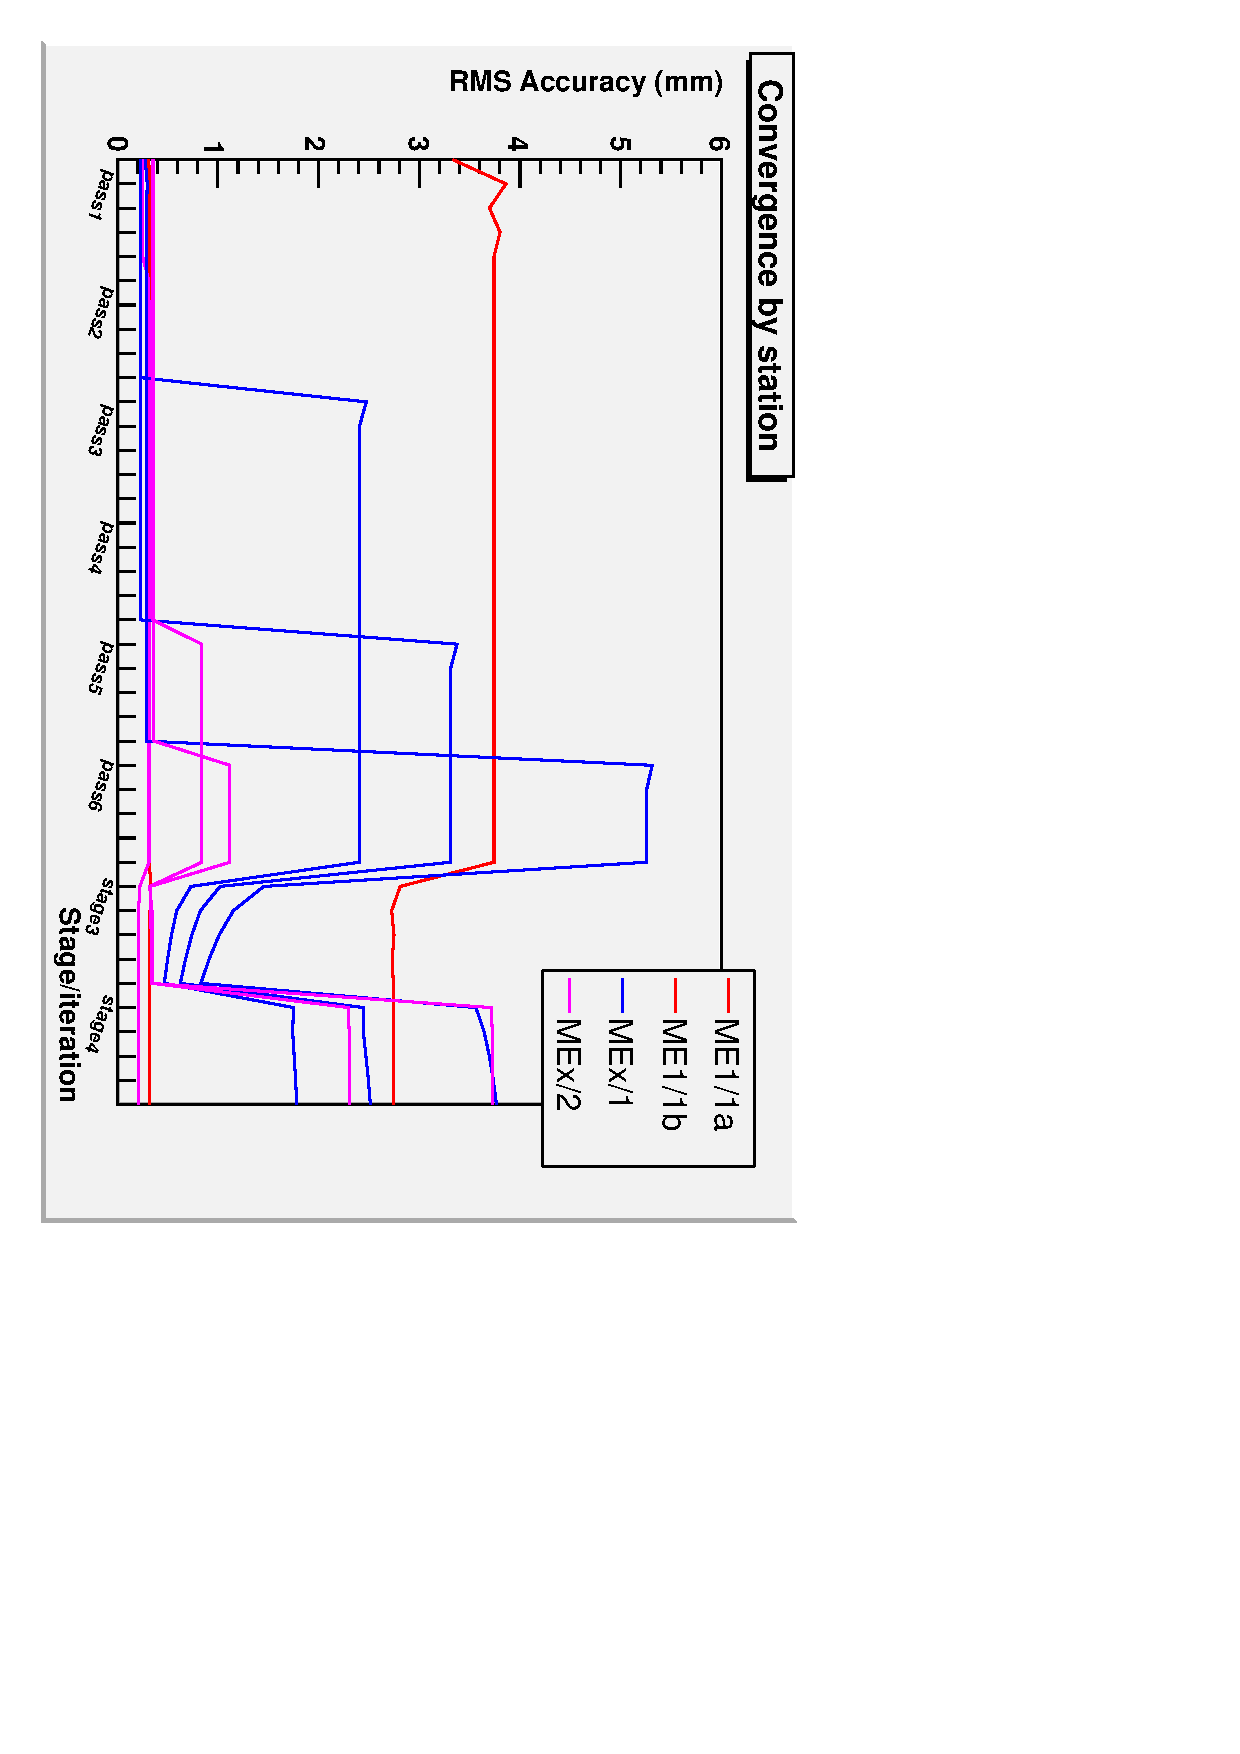
\includegraphics[height=\linewidth, angle=90]{convergence_endcap.pdf}
\end{columns}

\vfill
\begin{enumerate}
\item Pass1: same as ``infinite APEs'' (pre-alignment not on this plot)
\item Pass2: fix station 1 and steer tracks toward them, aligning station 2
\item Results in errors that compound as we go out
\item ``Stage 3'' is ``infinite APEs'' again (fixes everything)
\end{enumerate}

\vfill
This was the motivation for me to switch back to the ``infinite APEs'' method as our baseline.

\vfill
Apples-to-apples comparison (same starting misalignment) on next page.
\end{frame}

\begin{frame}
\frametitle{Scaling with $\int$luminosity}

\small

RMS of chamber residual misalignments within each station

(dashed grey line is $1/\sqrt{N}$ for comparison)

\vfill
\begin{columns}
\column{0.5\linewidth}
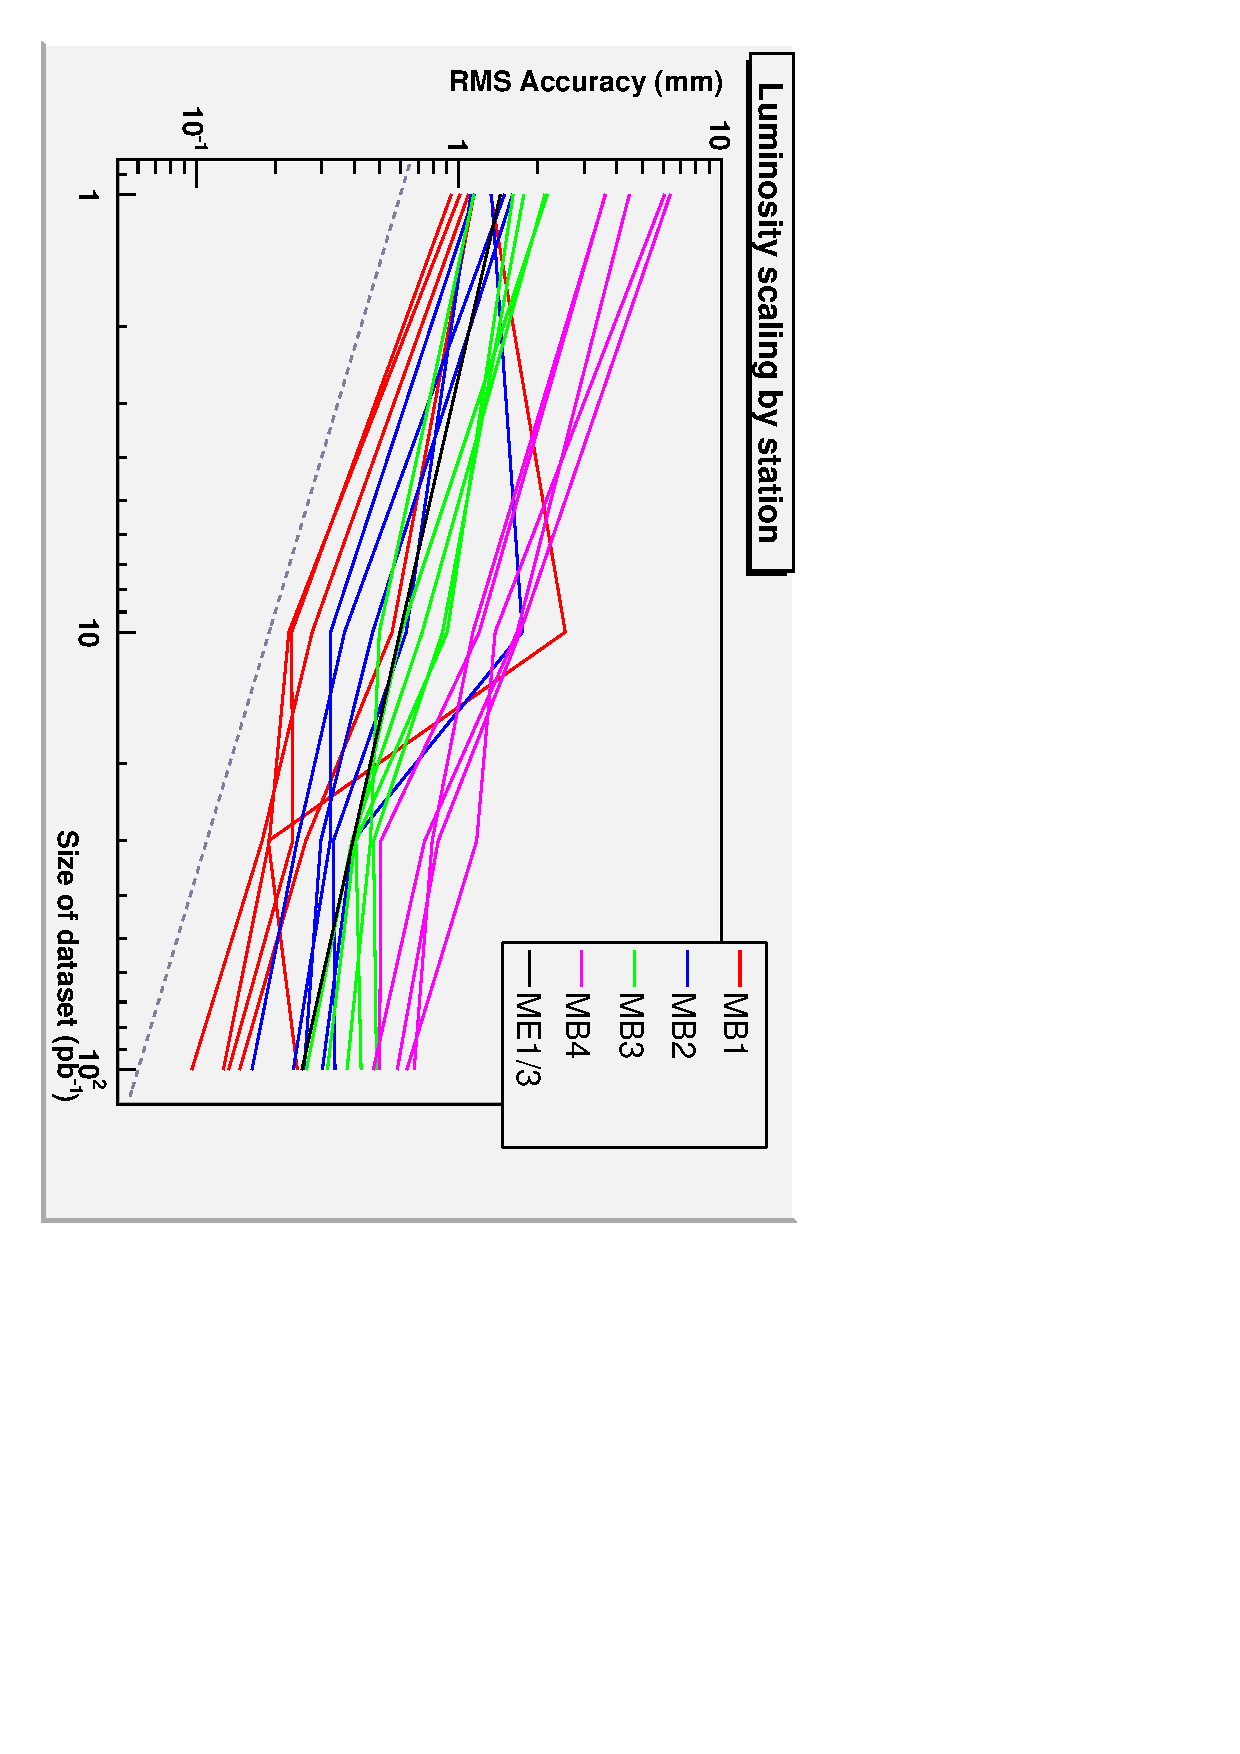
\includegraphics[height=0.9\linewidth, angle=90]{scaling_barrel.pdf}
\column{0.5\linewidth}
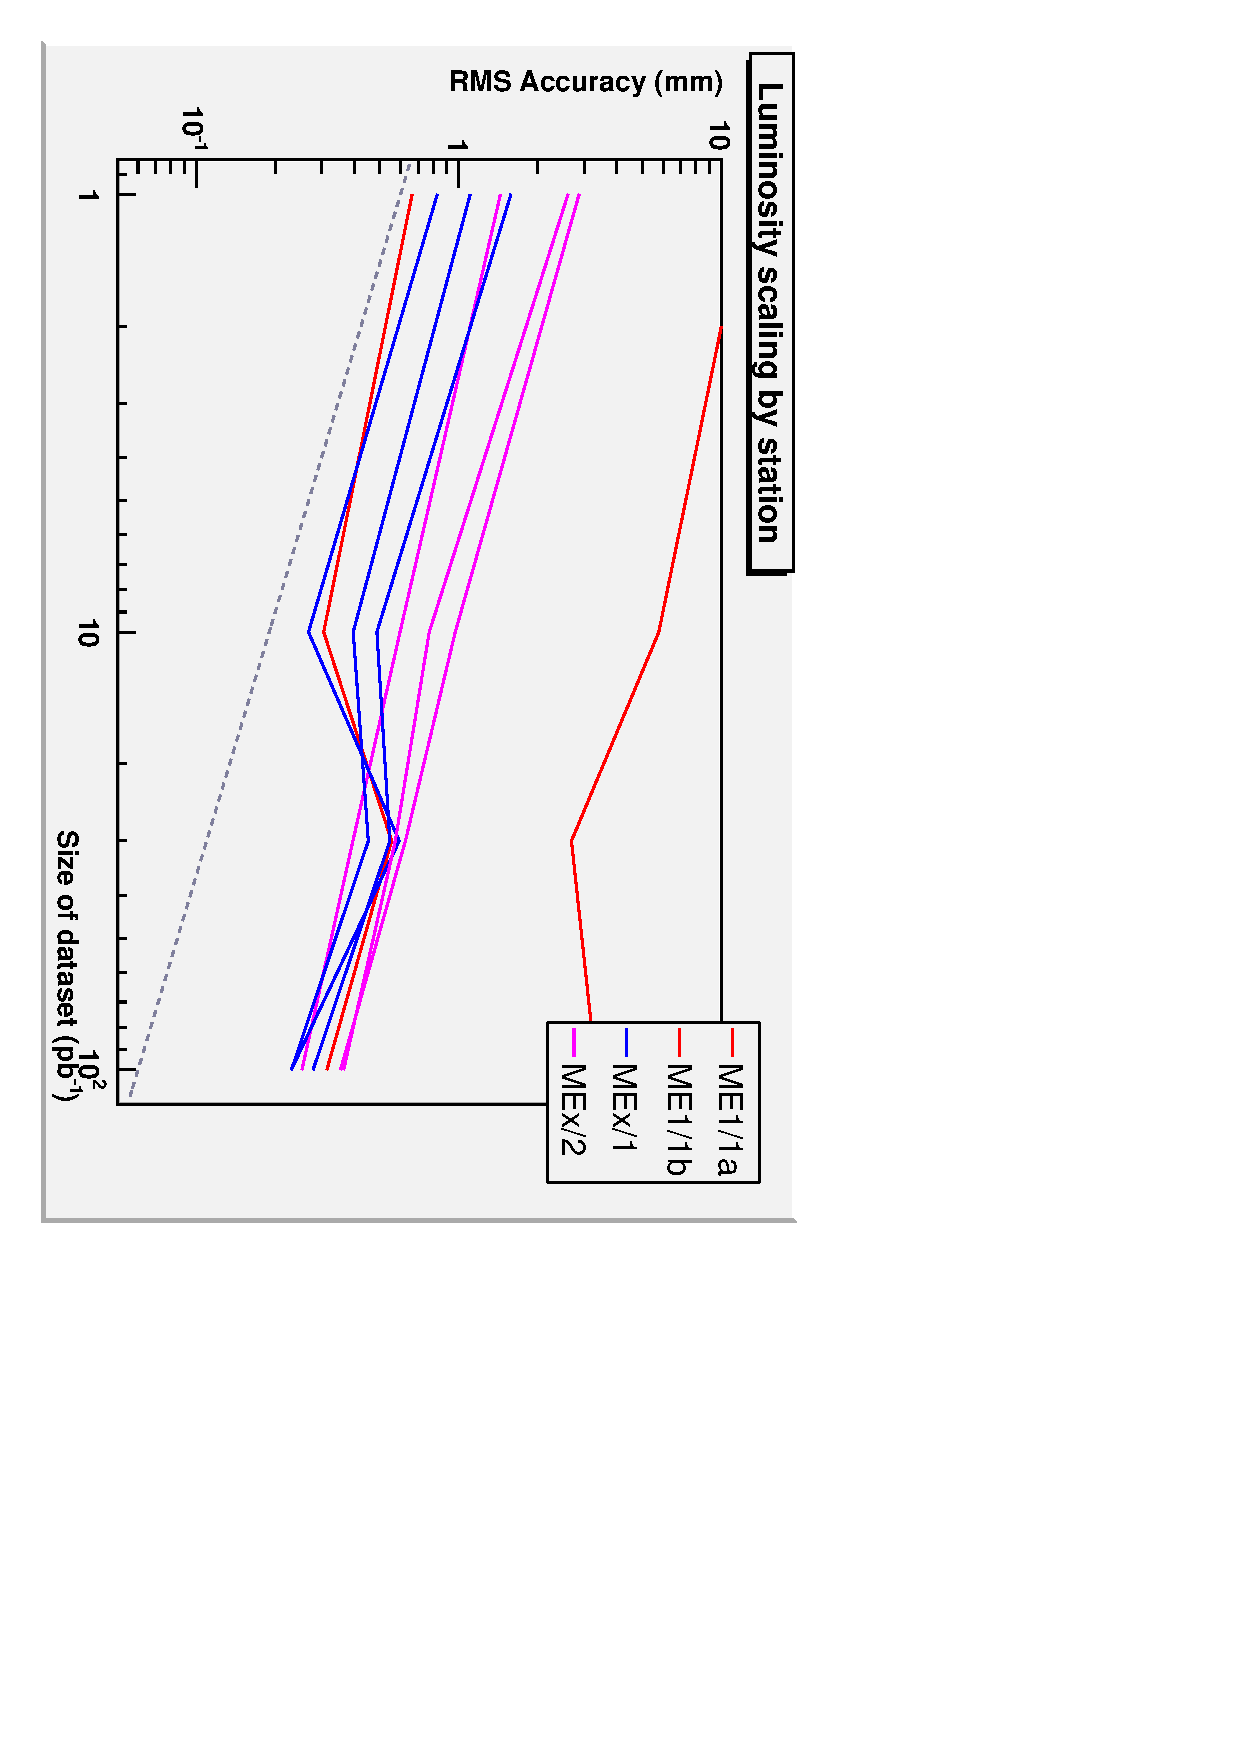
\includegraphics[height=0.9\linewidth, angle=90]{scaling_endcap.pdf}
\end{columns}

\vfill
Worst chamber within each station

\vfill
\begin{columns}
\column{0.5\linewidth}
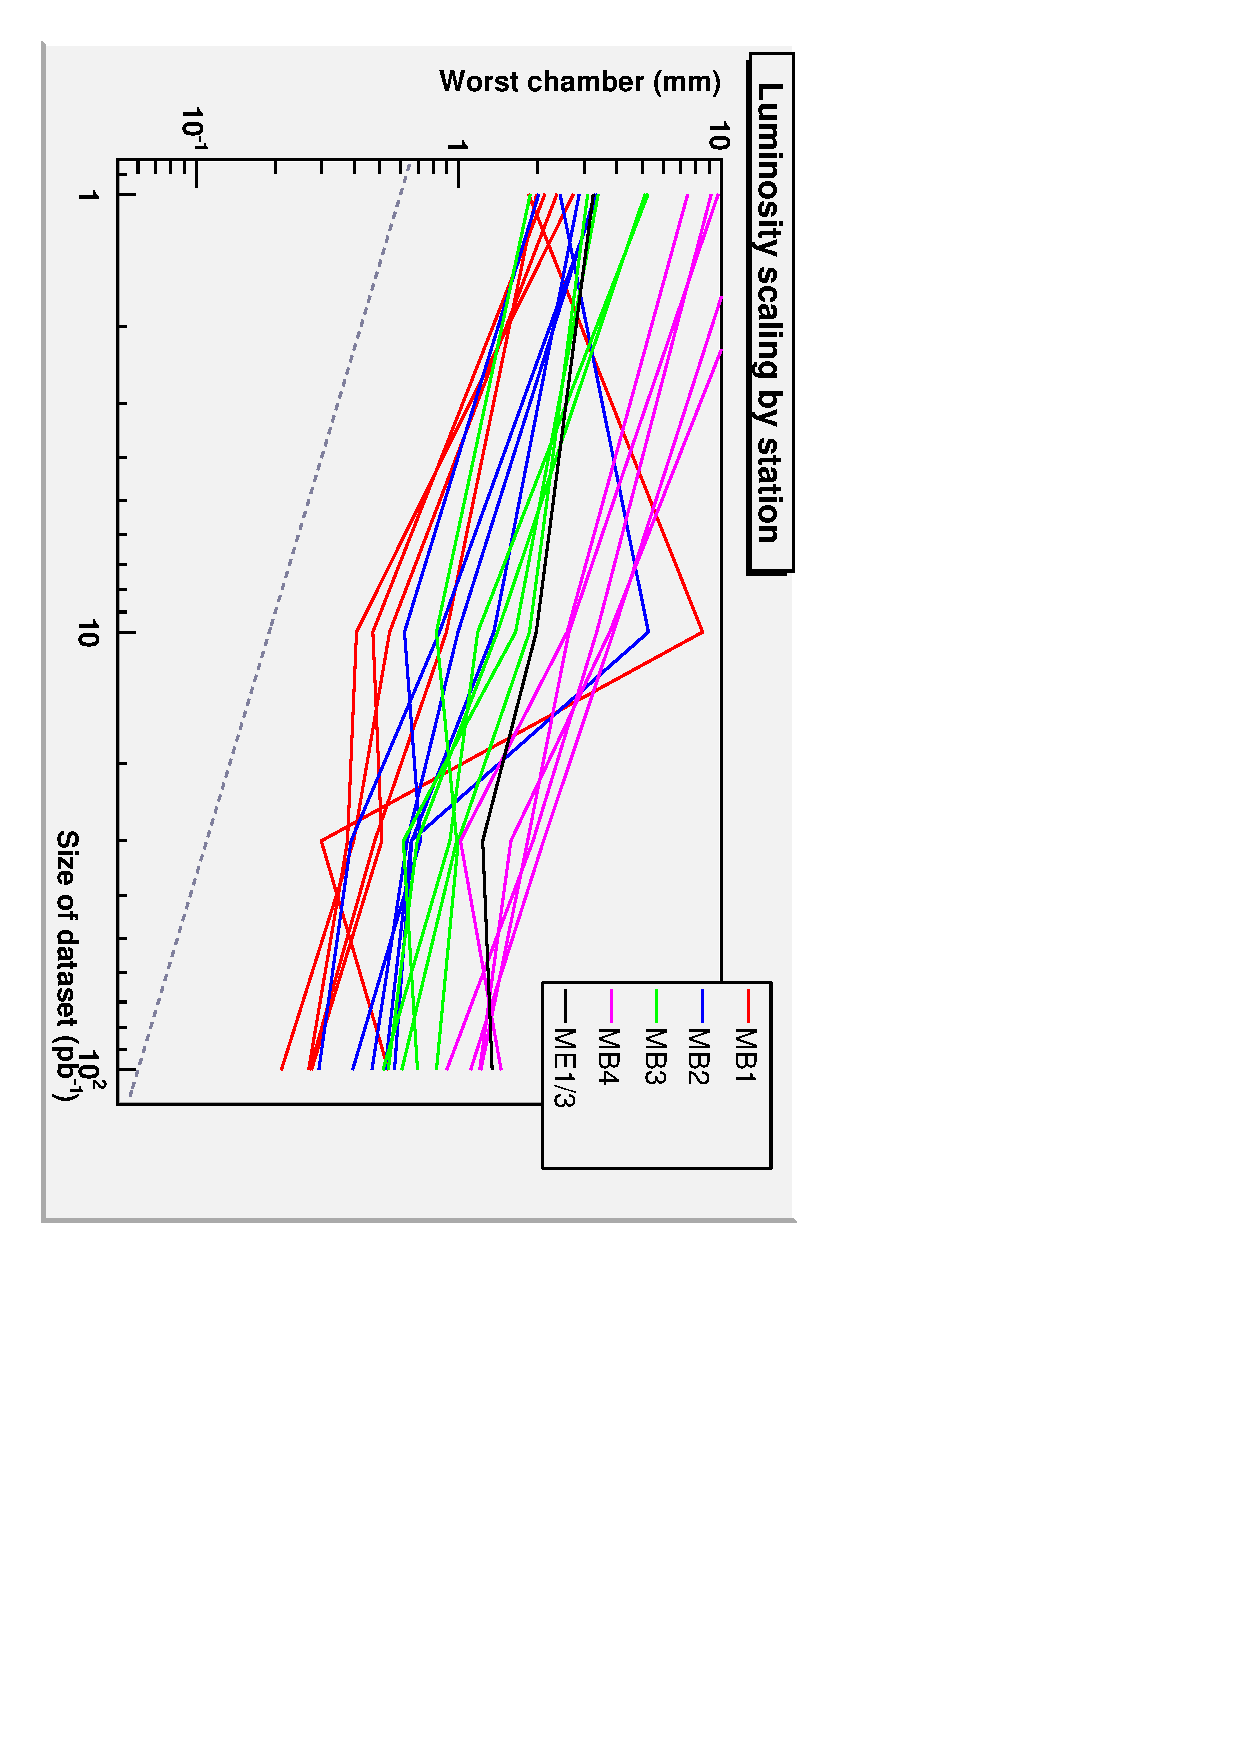
\includegraphics[height=0.9\linewidth, angle=90]{worst_barrel.pdf}
\column{0.5\linewidth}
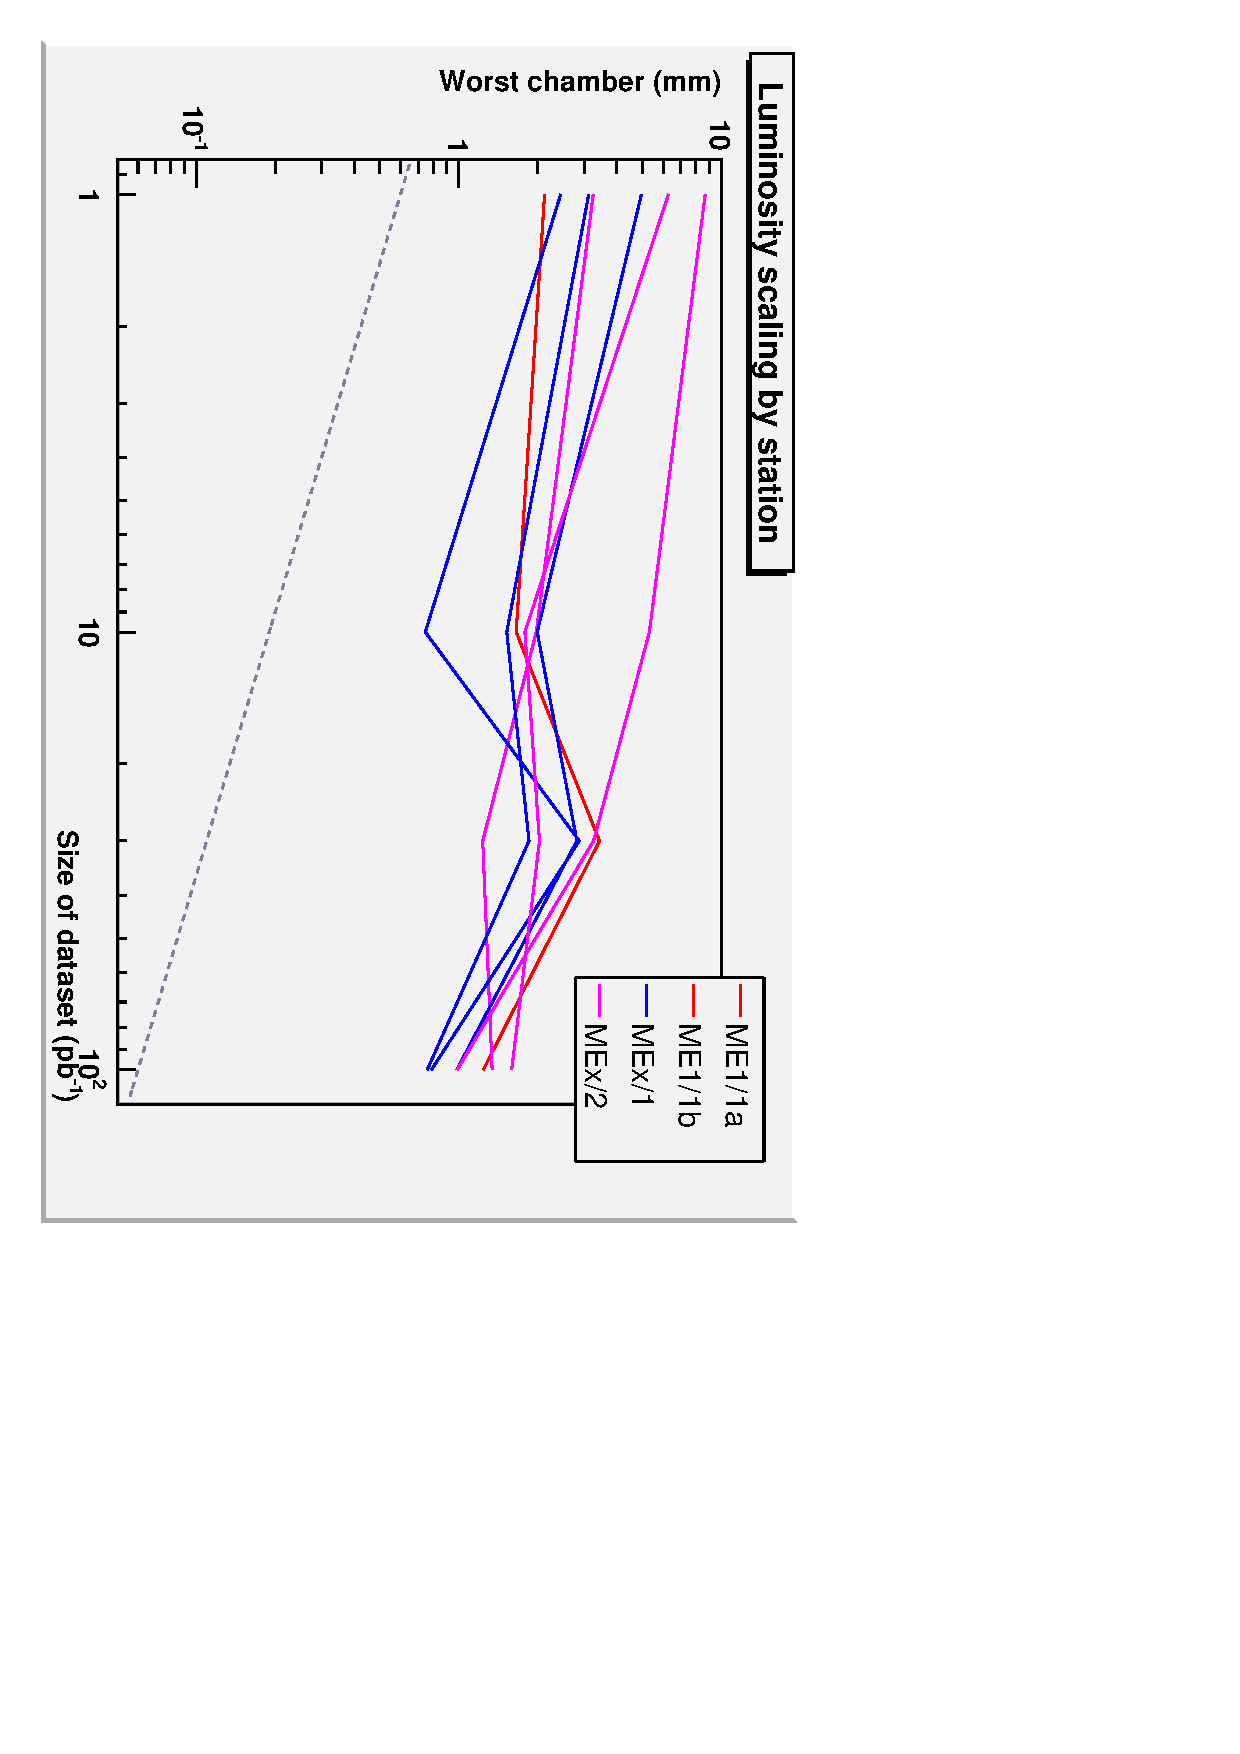
\includegraphics[height=0.9\linewidth, angle=90]{worst_endcap.pdf}
\end{columns}
\end{frame}

\begin{frame}
\frametitle{Consistency}

\small
\begin{itemize}
\item Within the ``infinite APE'' method, I still see differences (compare
slide 13 with slides 6--9)
\item My old studies used huge misalignments as a starting misalignment ($\sim$cm), and so do the last two slides
\item iCSA08 starting point is 0~$pb^{-1}$ scenario, which is closer
to reality, but has no layer misalignments (neither did the old
starting point, it turns out)
\item Quick study: RMS resolution per station with varying layer misalignment
\end{itemize}

\tiny
\begin{tabular}{c c c c}
station & with perfect layers (mm) & with 1$\times$ expected (mm) & with 2$\times$ expected (mm) \\\hline
MB 1 & 0.184 & 0.188 & 0.212 \\
MB 2 & 0.220 & 0.219 & 0.239 \\
MB 3 & 0.294 & 0.318 & 0.357 \\
MB 4 & 0.613 & 0.608 & 0.621 \\
ME1/1 & 0.227 & 0.216 & 0.247 \\
ME1/2 & 0.245 & 0.262 & 0.308 \\
ME1/3 & 0.679 & 0.678 & 0.686 \\
ME1/4 & 0.235 & 0.259 & 0.299 \\
ME2/1 & 0.149 & 0.171 & 0.218 \\
ME2/2 & 0.397 & 0.400 & 0.422 \\
ME3/1 & 0.213 & 0.224 & 0.260 \\
ME3/2 & 0.396 & 0.391 & 0.395 \\
ME4/1 & 0.267 & 0.302 & 0.358 \\
\end{tabular}

(DTs assumed to be 100~$\mu$m (guess), CSCs known from MTCC)
\end{frame}

\begin{frame}
\frametitle{Overlaps procedure}

\small
\begin{itemize}
\item Reminder: using tracks from CSC overlap regions, we fit to even-numbered chambers, align odds, then alternate
\item Problem: this is affected by devious tracks!  (small region of hits with non-infinite APEs, inward-out versus outward-in is not as well defined\ldots)
\item Test: rotate muon system; procedure should {\it not} be able to find its way back to ideal because the procedure only knows about relative information
\end{itemize}

\mbox{ } \hfill 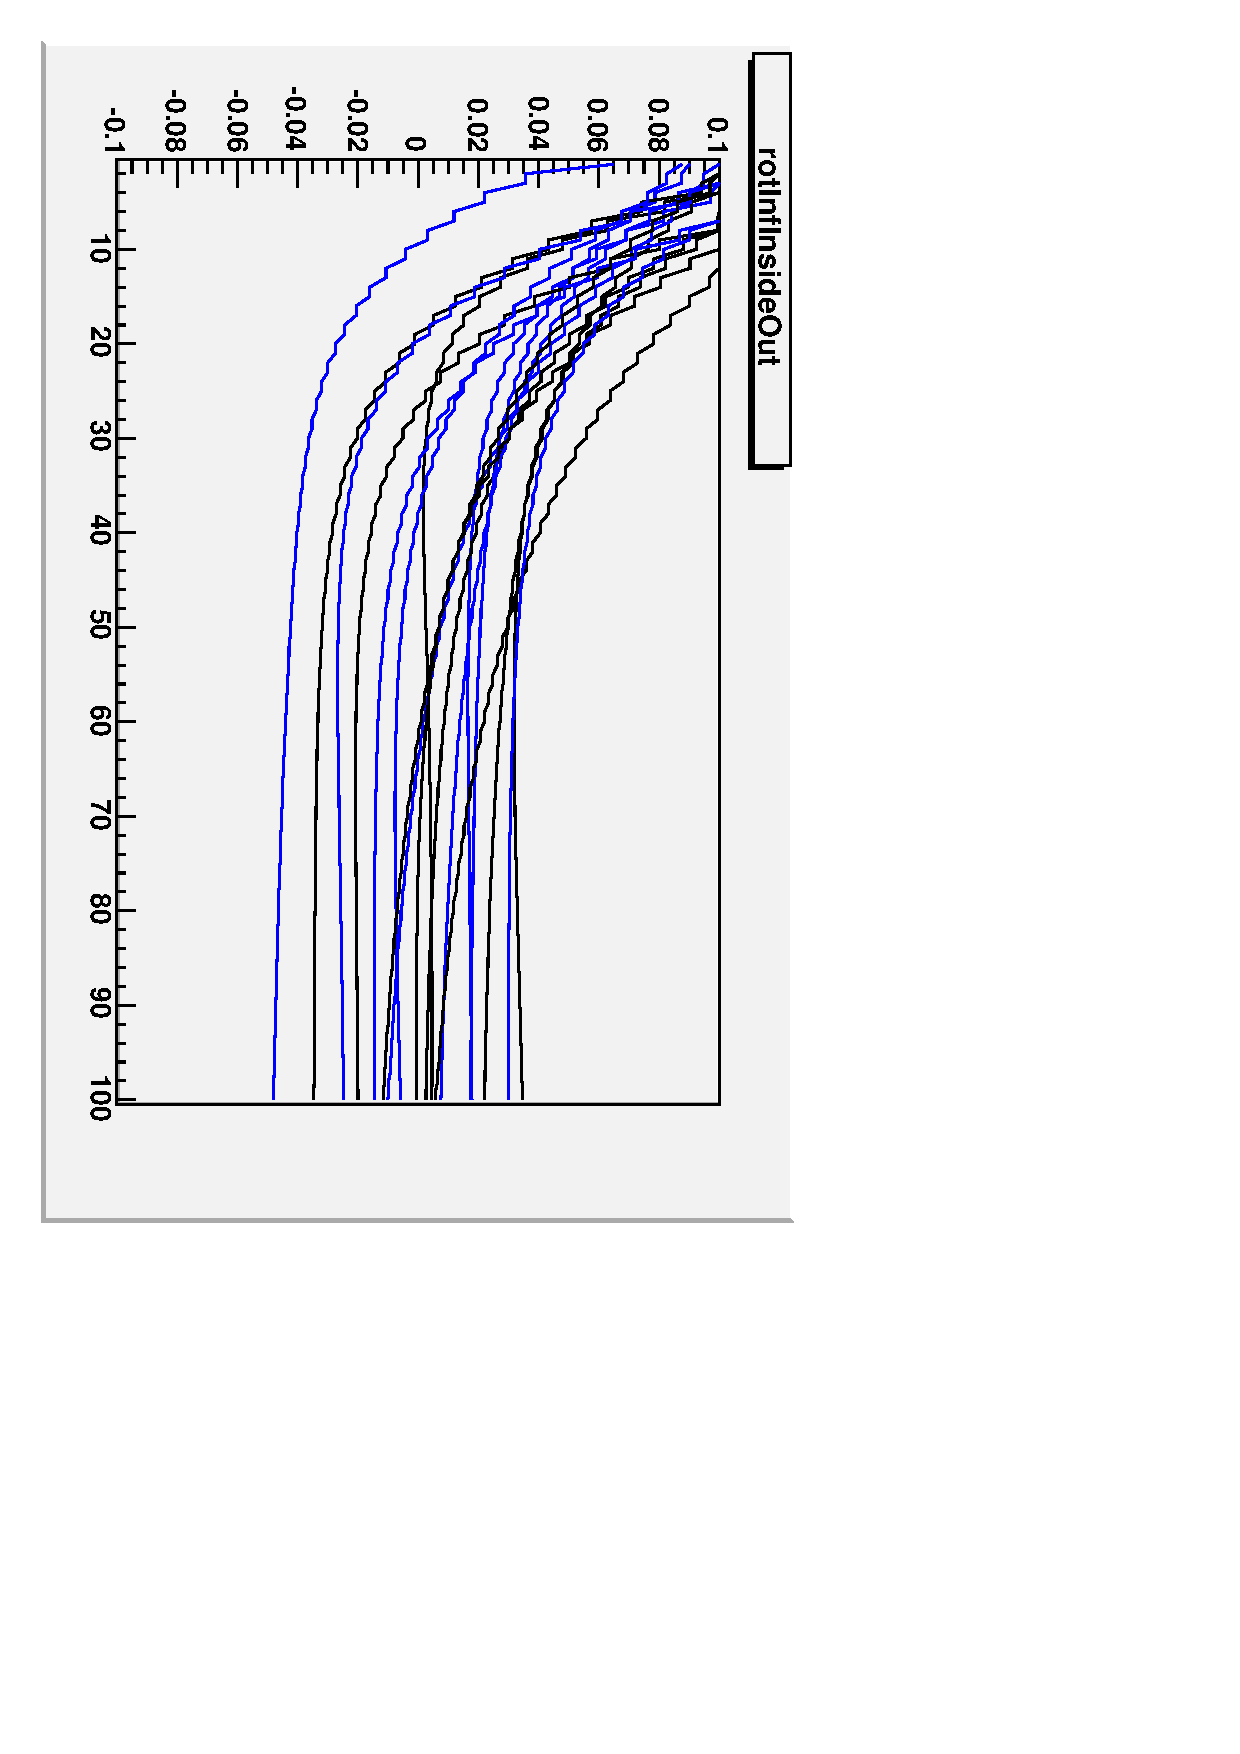
\includegraphics[height=0.6\linewidth, angle=90]{affected_by_bug.pdf} \hfill \mbox{ }
\end{frame}

\begin{frame}
\frametitle{Conclusions}

\small
\begin{itemize}\setlength{\itemsep}{0.1 cm}
\item Baseline procedure is in good shape: it should be the ``infinite APEs'' version.
\item This is what will go into iCSA08, and I've done many tests to be
sure it will be a successful and realistic test.
\item Overlaps procedure is still a work in progress: triggers, AlCa
paths, are all in place$^*$ and will deliver events in CSA and data, but
we don't know how to use them yet
\item ($^*$ caveat: CSA will deliver overlap globalMuons instead of
standAloneMuons, the mistake was caught too late)
\item Working on a track refitter that is immune to ``devious tracks''
bug, and uses only information I understand well (linear fits in the
overlap region, which Gena recommends); I would say it's 80\% there
\item Overlaps will be important for beam-halo {\it and} cosmic rays,
so it's something to fix very soon.  However, we never said that
success in iCSA08 depends on this part of the procedure (I made that
clear a month ago\ldots)
\end{itemize}
\label{numpages}
\end{frame}

%% \section*{First section}
%% \begin{frame}
%% \begin{center}
%% \Huge \textcolor{blue}{First section}
%% \end{center}
%% \end{frame}

\end{document}
